\documentclass{standalone}
\usepackage{tikz}
\usetikzlibrary{patterns, positioning}

\begin{document}
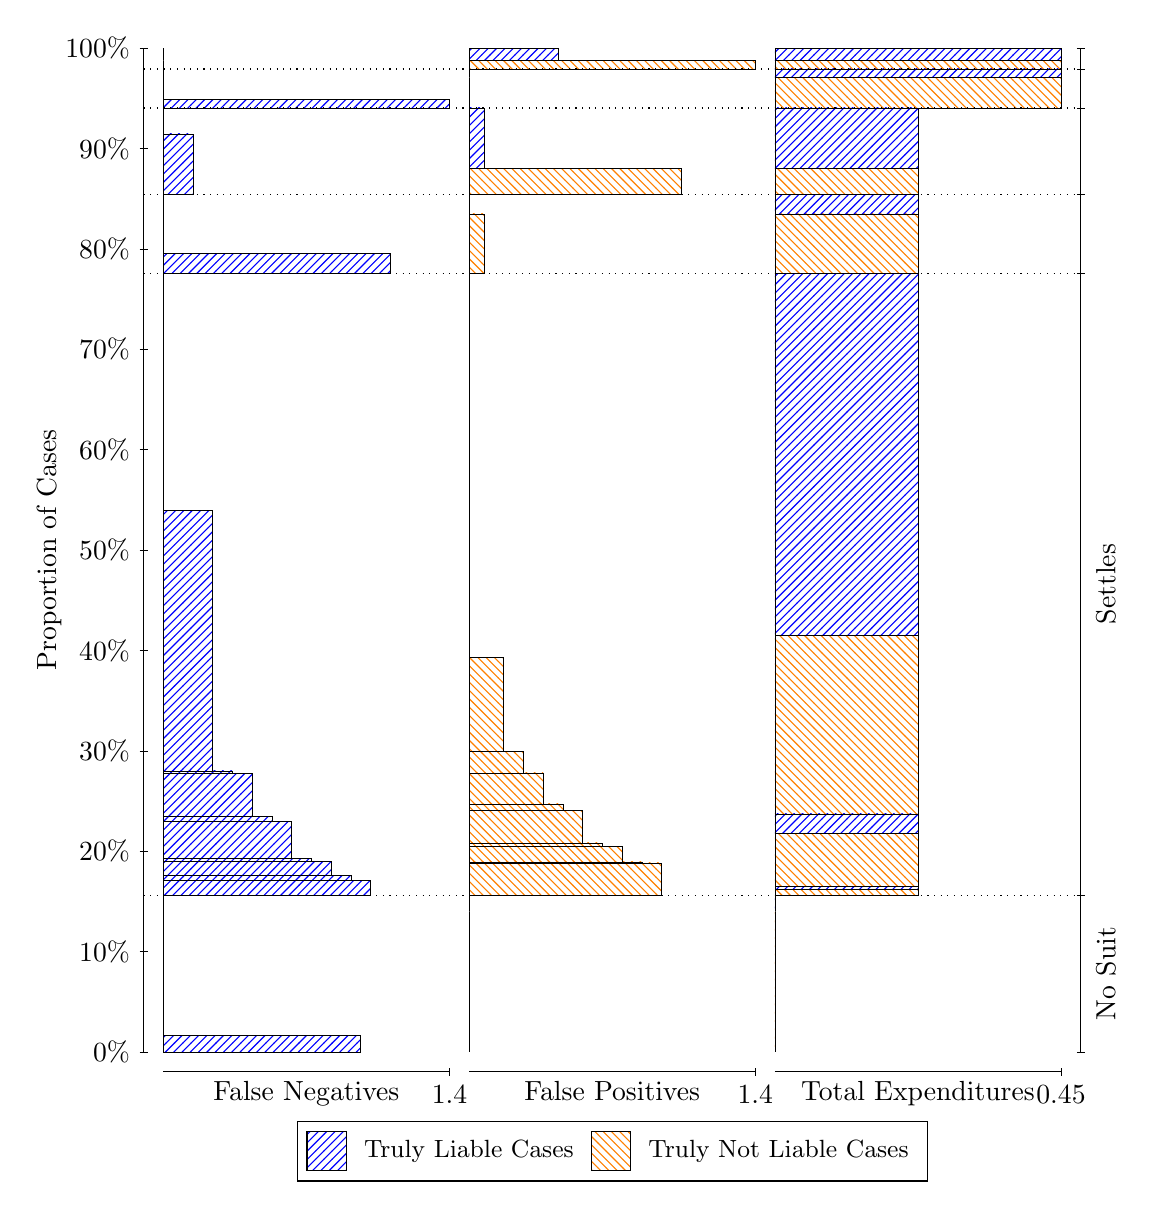
\begin{tikzpicture}
\draw[black, very thin] (1.5,1.75) -- (1.5,14.5);
\node[rotate=90, anchor=center] at (0.3, 8.125) {Proportion of Cases};
\draw[black, very thin] (1.45,1.75) -- (1.55,1.75);
\node[anchor=east] at (1.45, 1.75) {0\%};
\draw[black, very thin] (1.45,3.025) -- (1.55,3.025);
\node[anchor=east] at (1.45, 3.025) {10\%};
\draw[black, very thin] (1.45,4.3) -- (1.55,4.3);
\node[anchor=east] at (1.45, 4.3) {20\%};
\draw[black, very thin] (1.45,5.575) -- (1.55,5.575);
\node[anchor=east] at (1.45, 5.575) {30\%};
\draw[black, very thin] (1.45,6.85) -- (1.55,6.85);
\node[anchor=east] at (1.45, 6.85) {40\%};
\draw[black, very thin] (1.45,8.125) -- (1.55,8.125);
\node[anchor=east] at (1.45, 8.125) {50\%};
\draw[black, very thin] (1.45,9.4) -- (1.55,9.4);
\node[anchor=east] at (1.45, 9.4) {60\%};
\draw[black, very thin] (1.45,10.675) -- (1.55,10.675);
\node[anchor=east] at (1.45, 10.675) {70\%};
\draw[black, very thin] (1.45,11.95) -- (1.55,11.95);
\node[anchor=east] at (1.45, 11.95) {80\%};
\draw[black, very thin] (1.45,13.225) -- (1.55,13.225);
\node[anchor=east] at (1.45, 13.225) {90\%};
\draw[black, very thin] (1.45,14.5) -- (1.55,14.5);
\node[anchor=east] at (1.45, 14.5) {100\%};

\draw[black, very thin] (13.4,1.75) -- (13.4,14.5);
\draw[black, very thin] (13.35,1.75) -- (13.45,1.75);
\node[anchor=west] at (13.35, 1.75) {};
\draw[black, very thin] (13.35,3.7428) -- (13.45,3.7428);
\node[anchor=west] at (13.35, 3.7428) {};
\draw[black, very thin] (13.35,11.641) -- (13.45,11.641);
\node[anchor=west] at (13.35, 11.641) {};
\draw[black, very thin] (13.35,12.641) -- (13.45,12.641);
\node[anchor=west] at (13.35, 12.641) {};
\draw[black, very thin] (13.35,13.739) -- (13.45,13.739);
\node[anchor=west] at (13.35, 13.739) {};
\draw[black, very thin] (13.35,14.234) -- (13.45,14.234);
\node[anchor=west] at (13.35, 14.234) {};
\draw[black, very thin] (13.35,14.5) -- (13.45,14.5);
\node[anchor=west] at (13.35, 14.5) {};

\draw[black, very thin, pattern color=blue, pattern=north east lines] (1.75,1.75) rectangle (4.2557,1.9597);
\draw[black, very thin, pattern color=orange, pattern=north west lines] (1.75,1.9597) rectangle (1.75,3.7428);
\draw[black, very thin, pattern color=blue, pattern=north east lines] (1.75,3.7428) rectangle (4.381,3.9313);
\draw[black, very thin, pattern color=blue, pattern=north east lines] (1.75,3.9313) rectangle (4.1305,3.9967);
\draw[black, very thin, pattern color=blue, pattern=north east lines] (1.75,3.9967) rectangle (3.8799,4.1718);
\draw[black, very thin, pattern color=blue, pattern=north east lines] (1.75,4.1718) rectangle (3.6293,4.2112);
\draw[black, very thin, pattern color=blue, pattern=north east lines] (1.75,4.2112) rectangle (3.3787,4.6779);
\draw[black, very thin, pattern color=blue, pattern=north east lines] (1.75,4.6779) rectangle (3.1282,4.743);
\draw[black, very thin, pattern color=blue, pattern=north east lines] (1.75,4.743) rectangle (2.8776,5.2878);
\draw[black, very thin, pattern color=blue, pattern=north east lines] (1.75,5.2878) rectangle (2.627,5.3187);
\draw[black, very thin, pattern color=blue, pattern=north east lines] (1.75,5.3187) rectangle (2.3764,8.6237);
\draw[black, very thin, pattern color=orange, pattern=north west lines] (1.75,8.6237) rectangle (1.75,11.641);
\draw[black, very thin, pattern color=blue, pattern=north east lines] (1.75,11.641) rectangle (4.6316,11.89);
\draw[black, very thin, pattern color=orange, pattern=north west lines] (1.75,11.89) rectangle (1.75,12.641);
\draw[black, very thin, pattern color=blue, pattern=north east lines] (1.75,12.641) rectangle (2.1259,13.41);
\draw[black, very thin, pattern color=orange, pattern=north west lines] (1.75,13.41) rectangle (1.75,13.739);
\draw[black, very thin, pattern color=blue, pattern=north east lines] (1.75,13.739) rectangle (5.3833,13.848);
\draw[black, very thin, pattern color=orange, pattern=north west lines] (1.75,13.848) rectangle (1.75,14.234);
\draw[black, very thin, pattern color=orange, pattern=north west lines] (1.75,14.234) rectangle (1.75,14.342);
\draw[black, very thin, pattern color=blue, pattern=north east lines] (1.75,14.342) rectangle (1.75,14.5);
\draw[black, very thin, pattern color=orange, pattern=north west lines] (5.6333,1.75) rectangle (5.6333,3.5332);
\draw[black, very thin, pattern color=blue, pattern=north east lines] (5.6333,3.5332) rectangle (5.6333,3.7428);
\draw[black, very thin, pattern color=orange, pattern=north west lines] (5.6333,3.7428) rectangle (8.0764,4.1507);
\draw[black, very thin, pattern color=orange, pattern=north west lines] (5.6333,4.1507) rectangle (7.8259,4.1647);
\draw[black, very thin, pattern color=orange, pattern=north west lines] (5.6333,4.1647) rectangle (7.5753,4.363);
\draw[black, very thin, pattern color=orange, pattern=north west lines] (5.6333,4.363) rectangle (7.3247,4.4068);
\draw[black, very thin, pattern color=orange, pattern=north west lines] (5.6333,4.4068) rectangle (7.0741,4.8206);
\draw[black, very thin, pattern color=orange, pattern=north west lines] (5.6333,4.8206) rectangle (6.8236,4.8912);
\draw[black, very thin, pattern color=orange, pattern=north west lines] (5.6333,4.8912) rectangle (6.8236,4.901);
\draw[black, very thin, pattern color=orange, pattern=north west lines] (5.6333,4.901) rectangle (6.573,5.2938);
\draw[black, very thin, pattern color=orange, pattern=north west lines] (5.6333,5.2938) rectangle (6.3224,5.5714);
\draw[black, very thin, pattern color=orange, pattern=north west lines] (5.6333,5.5714) rectangle (6.0718,6.7605);
\draw[black, very thin, pattern color=blue, pattern=north east lines] (5.6333,6.7605) rectangle (5.6333,11.641);
\draw[black, very thin, pattern color=orange, pattern=north west lines] (5.6333,11.641) rectangle (5.8213,12.393);
\draw[black, very thin, pattern color=blue, pattern=north east lines] (5.6333,12.393) rectangle (5.6333,12.641);
\draw[black, very thin, pattern color=orange, pattern=north west lines] (5.6333,12.641) rectangle (8.327,12.97);
\draw[black, very thin, pattern color=blue, pattern=north east lines] (5.6333,12.97) rectangle (5.8213,13.739);
\draw[black, very thin, pattern color=orange, pattern=north west lines] (5.6333,13.739) rectangle (5.6333,14.125);
\draw[black, very thin, pattern color=blue, pattern=north east lines] (5.6333,14.125) rectangle (5.6333,14.234);
\draw[black, very thin, pattern color=orange, pattern=north west lines] (5.6333,14.234) rectangle (9.2667,14.342);
\draw[black, very thin, pattern color=blue, pattern=north east lines] (5.6333,14.342) rectangle (6.7609,14.5);
\draw[black, very thin, pattern color=orange, pattern=north west lines] (9.5167,1.75) rectangle (9.5167,3.5332);
\draw[black, very thin, pattern color=blue, pattern=north east lines] (9.5167,3.5332) rectangle (9.5167,3.7428);
\draw[black, very thin, pattern color=orange, pattern=north west lines] (9.5167,3.7428) rectangle (11.333,3.8134);
\draw[black, very thin, pattern color=blue, pattern=north east lines] (9.5167,3.8134) rectangle (11.333,3.8507);
\draw[black, very thin, pattern color=orange, pattern=north west lines] (9.5167,3.8507) rectangle (11.333,4.5309);
\draw[black, very thin, pattern color=blue, pattern=north east lines] (9.5167,4.5309) rectangle (11.333,4.7735);
\draw[black, very thin, pattern color=orange, pattern=north west lines] (9.5167,4.7735) rectangle (11.333,7.0404);
\draw[black, very thin, pattern color=blue, pattern=north east lines] (9.5167,7.0404) rectangle (11.333,11.641);
\draw[black, very thin, pattern color=orange, pattern=north west lines] (9.5167,11.641) rectangle (11.333,12.393);
\draw[black, very thin, pattern color=blue, pattern=north east lines] (9.5167,12.393) rectangle (11.333,12.641);
\draw[black, very thin, pattern color=orange, pattern=north west lines] (9.5167,12.641) rectangle (11.333,12.97);
\draw[black, very thin, pattern color=blue, pattern=north east lines] (9.5167,12.97) rectangle (11.333,13.739);
\draw[black, very thin, pattern color=orange, pattern=north west lines] (9.5167,13.739) rectangle (13.15,14.125);
\draw[black, very thin, pattern color=blue, pattern=north east lines] (9.5167,14.125) rectangle (13.15,14.234);
\draw[black, very thin, pattern color=orange, pattern=north west lines] (9.5167,14.234) rectangle (13.15,14.342);
\draw[black, very thin, pattern color=blue, pattern=north east lines] (9.5167,14.342) rectangle (13.15,14.5);
\draw[black, dotted] (1.5,3.7428) -- (13.4,3.7428);
\draw[black, dotted] (1.5,11.641) -- (13.4,11.641);
\draw[black, dotted] (1.5,12.641) -- (13.4,12.641);
\draw[black, dotted] (1.5,13.739) -- (13.4,13.739);
\draw[black, dotted] (1.5,14.234) -- (13.4,14.234);
\draw[black, very thin] (1.75,1.5) -- (5.3833,1.5);
\node[anchor=north] at (3.5667, 1.5) {False Negatives};
\draw[black, very thin] (5.3833,1.45) -- (5.3833,1.55);
\node[anchor=north] at (5.3833, 1.45) {1.4};

\draw[black, very thin] (5.6333,1.5) -- (9.2667,1.5);
\node[anchor=north] at (7.45, 1.5) {False Positives};
\draw[black, very thin] (9.2667,1.45) -- (9.2667,1.55);
\node[anchor=north] at (9.2667, 1.45) {1.4};

\draw[black, very thin] (9.5167,1.5) -- (13.15,1.5);
\node[anchor=north] at (11.333, 1.5) {Total Expenditures};
\draw[black, very thin] (13.15,1.45) -- (13.15,1.55);
\node[anchor=north] at (13.15, 1.45) {0.45};

\node[black, centered, rotate=90] at (13.72, 2.7464) {No Suit};
\node[black, centered, rotate=90] at (13.72, 7.6921) {Settles};





\draw (7.449999999999999,1.5) node[draw=none] (baseCoordinate) {};
\begin{scope}[align=center]
        \matrix[scale=0.5, draw=black, below=0.5cm of baseCoordinate, nodes={draw}, column sep=0.1cm]{
            \node[rectangle, draw, minimum width=0.5cm, minimum height=0.5cm, pattern=north east lines, pattern color=blue] {}; &
            \node[draw=none, font=\small] (B) {Truly Liable Cases}; &
            \node[rectangle, draw, minimum width=0.5cm, minimum height=0.5cm, pattern=north west lines, pattern color=orange] {}; &
            \node[draw=none, font=\small] (B) {Truly Not Liable Cases}; \\
            };
\end{scope}

\end{tikzpicture}
\end{document}